\begin{frame}[allowframebreaks]{Control - General explanation}
    Instead of using GPS set-points, provide the agent with language and the goal of keeping the surprise pose as low as 0.1 while avoiding collisions with the walls. Numerical values will be refined later.


    Flight controller: PX4 (Software)

    FCU: Pixhawk4 (Hardware)


    \section{Goal (set-point)}
        A composite goal must be provided to the planner and should include:

        Keep the surprise pose as low as possible in the controller cost function.


    \section{Cost function}

        The cost function in the model predictive controller (MPC)
        \[
            J = \sum_{k=0}^{N-1} \left[ \left( x_k - x_k^{\mathrm{ref}} \right)^T Q \left( x_k - x_k^{\mathrm{ref}} \right) + u_k^T R u_k \right]
        \]

         X is the Wasserstein anomaly vector.

        \begin{figure}[H]
            \centering
            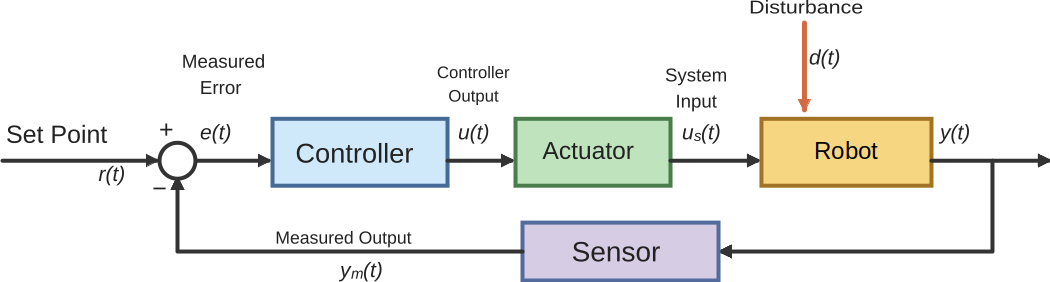
\includegraphics[width=0.9\textwidth]{a_typical_controller.png}
        \end{figure}

        Both drones use \textbf{MPC} to reach their next set-point

        Feedback system from a feedback that is formed of resource\_gain and goal\_gain
\end{frame}
